\documentclass[11pt, number, times, preprint]{article}
\setlength{\arrayrulewidth}{0.4mm}
\setlength{\tabcolsep}{10pt}
\renewcommand{\arraystretch}{1.2}

\usepackage[margin=1.7in]{geometry}

\usepackage{amsmath,amsfonts,amssymb,amsthm,epsfig,epstopdf,titling,url,array, pdflscape, fancyhdr, lastpage, tikz, hyperref}
\usepackage{blindtext}
\usepackage{dsfont}
\usepackage{caption}
\usepackage{subcaption}

\title{Skew Axial Algebras of Monster Type}
\author{Michael Turner\textsuperscript{}\thanks{\textsuperscript{}
School of Mathematics, University of Birmingham, Edgbaston, Birmingham, B15 2TT, UK, Email:
mxt187@student.bham.ac.uk
}}
\date{\today}

\newtheoremstyle{sltheorem}
{}                % Space above
{}                % Space below
{\slshape}        % Theorem body font % (default is "\upshape")
{}                % Indent amount
{\bfseries}       % Theorem head font % (default is \mdseries)
{.}               % Punctuation after theorem head % default: no punctuation
{ }               % Space after theorem head
{}                % Theorem head spec

\theoremstyle{sltheorem}
\newtheorem{thm}{Theorem}[section]
\newtheorem{lem}[thm]{Lemma}
\newtheorem{prop}[thm]{Proposition}
\newtheorem{cor}[thm]{Corollary}
\newtheorem*{thm*}{Theorem}
\newtheorem*{cor*}{Corollary}

\theoremstyle{definition}
\newtheorem{defn}[thm]{Definition}
\newtheorem{conj}[thm]{Conjecture}
\newtheorem{exmp}[thm]{Example}
\newtheorem{prob}[thm]{Problem}
\newtheorem{no}[thm]{Notation}
\newtheorem*{claim}{Claim}
\newtheorem*{claimpf}{Proof of claim}
\newtheorem*{step1}{Step 1}
\newtheorem*{step2}{Step 2}
\theoremstyle{remark}
\newtheorem*{rem}{Remark}
\newtheorem*{note}{Note}
\newtheorem*{ques}{Question}

\newcommand{\bb}[1]{\mathbb{#1}}
\newcommand{\id}{\mathds{1}}
\newcommand{\F}{\mathbb{F}}
\newcommand{\mcal}[1]{\mathcal{#1}}
\newcommand{\frk}[1]{\mathfrak{#1}}
\newcommand{\ad}[1]{\text{ad}_{#1}}
\newcommand{\Mod}[1]{\ (\mathrm{mod}\ #1)}
\newcommand{\Sy}[1]{\text{Sym}(#1)}
\newcommand{\Alt}[1]{\text{Alt}(#1)}
\newcommand{\Sp}[1]{\text{Sp}_{#1}}
\newcommand{\Orth}[1]{\text{O}_{#1}}
\newcommand{\SU}[1]{\text{SU}_{#1}}
\newcommand{\Fitwo}{\text{Fi}_{22}}
\newcommand{\Fithree}{\text{Fi}_{23}}
\newcommand{\Fifour}{\text{Fi}_{24}}
\newcommand{\GenG}[1]{\langle #1\rangle}
\newcommand{\GenA}[1]{\langle\!\langle #1\rangle\!\rangle}
\newcommand{\fustar}[1]{(\mcal{#1},\star)}
\newcommand{\fusast}[1]{(\mcal{#1},\ast)}
\newcommand{\fustarG}[1]{(#1,\star)}
\newcommand{\fusastG}[1]{(#1,\ast)}
\newcommand{\Z}{\mathbb{Z}}
\newcommand{\N}{\mathbb{N}}
\newcommand{\Q}{\mathbb{Q}}
\newcommand{\algQ}{\bar{\mathbb{Q}}}
\newcommand{\spec}[1]{\text{Spec}(#1)}
\newcommand{\ann}[1]{\text{Ann}(#1)}
\newcommand{\Span}[1]{\text{span}(#1)}
\newcommand{\Nil}[1]{\text{Nil}(#1)}
\newcommand{\ZI}{\mcal{N}}
\newcommand{\al}{\alpha}
\newcommand{\bt}{\beta}
\newcommand{\sg}{\sigma}
\newcommand{\lm}{\lambda}
\newcommand{\dt}{\delta}
\newcommand{\ep}{\epsilon}
\newcommand{\lmf}{\lambda^f}
\newcommand{\tu}[1]{\tau_{#1}}
\newcommand{\gm}{\gamma}
\newcommand{\te}{\theta}
\newcommand{\zt}{\zeta}
\newcommand{\kp}{\kappa}
\newcommand{\dual}[1]{#1^\dagger}
\newcommand{\ddual}[1]{{#1^\dagger}^\dagger}
\newcommand{\assoc}{\mcal{A}}
\newcommand{\jor}[1]{\mcal{J}(#1)}
\newcommand{\mon}[1]{\mcal{M}(#1)}
\newcommand{\Spec}[1]{\text{Spec}(#1)}
\newcommand{\Miy}[1]{\text{Miy}(#1)}
\newcommand{\hw}{\mcal{H}}
\newcommand{\hwc}{\hat{\mcal{H}}}
\newcommand{\TB}{2\text{B}}
\newcommand{\TA}{3\text{A}}
\newcommand{\TC}{3\text{C}}
\newcommand{\FA}{4\text{A}}
\newcommand{\FB}{4\text{B}}
\newcommand{\FJ}{4\text{J}}
\newcommand{\FY}{4\text{Y}}
\newcommand{\CA}{5\text{A}}
\newcommand{\SA}{6\text{A}}
\newcommand{\SJ}{6\text{J}}
\newcommand{\SY}{6\text{Y}}
\newcommand{\IY}[1]{\text{IY}_{#1}}
\providecommand{\keywords}[1]
{
  \small	
  \textbf{Keywords:} #1
}

\begin{document}
\maketitle
\begin{abstract}
%
Deformable image registration is a fundamental task in medical image analysis and plays a crucial role in a wide range of clinical applications. 
Recently, deep learning-based approaches have been widely studied for deformable medical image registration and achieved promising results. However, existing deep learning image registration techniques do not  theoretically guarantee %diffeomorphic 
topology-preserving transformations. This is a key property to preserve anatomical structures and achieve plausible transformations that can be used in real clinical settings.
%
We propose a novel framework for deformable image registration. Firstly, we introduce a  novel regulariser based on conformal-invariant properties in a nonlinear elasticity setting.
Our regulariser enforces  the deformation field  to be  smooth, invertible and orientation-preserving. %differentiable.  
More importantly, we strictly guarantee topology preservation yielding to a clinical meaningful registration.  Secondly, 
we boost the performance of our regulariser through coordinate MLPs, where one can view the to-be-registered images as continuously differentiable entities. 
We demonstrate, through numerical and visual experiments, that our framework is able to outperform current techniques for image registration.
%
\keywords{Homeomorphic image registration \and Lung CT \and Conformal invariant hyperelastic regularisation.}
%
\end{abstract}
% Importance and appeal of children's drawings
Children's depictions of the human figure are highly expressive and varied.
As one of the very first subjects children attempt to draw, the representation begins as an almost unintelligible cloud of scribbles. 
As the child grows, their representation of the human figure becomes more developed and is extended to graphically represent many different types of characters: people, animals, and even personified objects (see Figure 1).

Who among us has not wished, either as a child or as an adult, to see such figures come to life and move around on the page?
Sadly, while it is relatively fast to produce a single drawing, creating the sequence of images necessary for animation is a much more tedious endeavor, requiring discipline, skill, patience, and sometimes complicated software.
As a result, most of these figures remain static upon the page.

% We built a system to animate them.
Inspired by the importance and appeal of the drawn human figure, we design and build a system to automatically animate it given an in-the-wild photograph of a child's drawing. 
Our system is fast, intuitive, and robust to much of the variation present in these types of drawings, making it well-suited to allow our target audience--children--to see their own characters coming to life.
The system is comprised of four stages: figure detection, segmentation masking, pose estimation/rigging, and animation. 
We describe each stage and identify common causes of failure in each. 
For object detection and pose estimation, we make use of existing computer vision models designed to detect human figures and joints in photographs; we fine-tune these models for use with children's drawings.
For segmentation, we present a straightforward, image processing-based method that, for animation purposes, is more useful and accurate than segmentation masks obtained from a fine-tuned object detection model.
During the animation step, we take advantage of the \textit{twisted perspective} commonly seen in children’s drawings to retarget motion capture data onto the character in a novel and appealing way.

% We use existing machine learning models. However, given the wide domain gap it's not clear how much fine-tuning data was needed. So we ran some experiments to find out and report it.
While our system leverages existing models and techniques, most are not directly applicable to the task due to the many differences between photographic images and simple pen and paper representations. 
To this end, we couple the presentation of our system with a set of experiments exploring the relationship between fine-tuning training set size and success rates.
We also include a perceptual study validating viewer preference for incorporating \textit{twisted perspective} into the motion retargeting step.

We validate the desirability and appeal of our system by building and publicly releasing a version of it as the \AD Demo \,\cite{animateddrawings}.
Launched in December 2021, this demo has been used by millions of people around the world to animate their children's drawings.
Inspired by this reception, our second contribution is The Amateur Drawings Dataset: \hjs{180,000 drawings and user-accepted annotations collected, with consent, through the demo. See Section \ref{sec:UI} for a description of how the annotations were generated.}
We believe this dataset will be a resource to researchers from various fields seeking to better understand the space of amateur drawings, evaluate new algorithms in this domain, or develop new drawing-based tools in general.

To summarize, our contributions are as follows:
\begin{enumerate}
    \item 
    We explore the problem of automatic sketch-to-animation for children's drawings of human figures and present a framework that achieves this effect. We also present a set of experiments determining the amount of training data necessary to achieve high levels of success and a perceptual study validating the usefulness of our motion retargeting technique.
    \item To encourage additional research in the domain of amateur drawings, we present a first-of-its-kind dataset of 180,000 user-submitted amateur drawings, along with user-accepted bounding box, segmentation mask, and joint location annotations.
\end{enumerate}

Upon acceptance of this paper, we plan to publicly release the Amateur Drawings Dataset, project code, and fine-tuned model weights.

\section{Prerequisites}
\subsection{Axial Algebras}
Axial algebras have been defined in multiple papers so this section will be brief. For an in-depth discussion, we recommend to look at \cite{hall2015universal}, \cite{khasraw2020structure} and \cite{mcinroy2022axial}. A starting point is the definition of a fusion law in \cite{de2020decomposition}. 
\begin{defn}
Let $\mcal{F}$ be a set and let $\star: \mcal{F} \times \mcal{F} \rightarrow 2^{\mcal{F}}$ be a binary operator, where $2^{\mcal{F}}$ denotes the power set of $\mcal{F}$. We call the pair $\fustar{F}$, a \emph{fusion law}. We will refer to the fusion law by $\mcal{F}$. We say it is  \emph{symmetric} if for all $x,y\in \mcal{F}$, we have $x\star y=y\star x$.  
\end{defn}
For axial algebras, as they are commutative, fusion laws are considered to be symmetric. Given a fusion law, one is able to grade it using a group. We will denote group multiplication by juxtaposition. 
\begin{defn} Let $\fustar{F}$ be a fusion law and $T$ be a group. We say $\mcal{F}$ is $T$-graded if there exists a map $\xi: \mcal{F}\rightarrow T$
such that for $\lm, \mu\in \mcal{F}$,
$$\xi(\nu)=\xi(\lm)\xi(\mu)$$
for all $\nu\in \lm\star \mu$.
\end{defn}
\begin{table}[b]
\begin{minipage}{.5\linewidth}
\centering
\begin{tabular}{|c|c|c|c|} 
 \hline
  $\star$& 0 & 1 & $\eta$\\ [0.4ex] 
 \hline
 0 & 0 &  & $\eta$\\ 
 \hline
 1 &  & 1 & $\eta$\\
 \hline
 $\eta$ & $\eta$ & $\eta$& 1, 0\\
 \hline
\end{tabular}
\caption{Fusion law of $\jor{\eta}$}\label{J Table}
\end{minipage}%
\begin{minipage}{.5\linewidth}
\centering
\begin{tabular}{|c|c|c|c|c|} 
 \hline
  $\star$& 0 & 1 & $\alpha$ & $\beta$\\ [0.4ex] 
 \hline
 0 & 0 &  & $\alpha$ & $\beta$\\ 
 \hline
 1 &  & 1 & $\alpha$ & $\beta$\\
 \hline
 $\alpha$ & $\alpha$ & $\alpha$& 1, 0 & $\beta$\\
 \hline
 $\beta$ & $\beta$ & $\beta$ & $\beta$ & 1, 0, $\alpha$\\
 \hline
 \end{tabular}
 \caption{Fusion law of $\mon{\al,\bt}$}
 \label{M Table}
 \end{minipage}
\end{table}
The fusion laws that are used in this paper are $\jor{\eta}$ and $\mon{\al,\bt}$, which are defined in Tables \ref{J Table} and \ref{M Table} respectively. Let $C_2=\{e,s\}$ be the cyclic group of order two, where $e$ is the identity element. Then $\jor{\eta}$ and $\mon{\al,\bt}$ are both $C_2$-graded with $0$, $1$, $\al$ are mapped to the $e$ and $\eta$, $\bt$ are mapped to $s$.

Let $A$ be a commutative algebra over $\F$. For $a\in A$, the adjoint map of $a$ is $\text{ad}_a: A \rightarrow A$ with $\text{ad}_a(x)=ax$ for all $x\in A$. Let $\text{Spec}(a)$ be the set of eigenvalues of $\text{ad}_a$ and for $\lambda \in \F$, let $A_{\lambda}(a)$ be the $\lambda$-eigenspace of $\text{ad}_a$. Note that $A_\lambda(a)$ is non-zero if and only if $\lambda \in \spec{a}$. We write for $S\subseteq \F$, $A_S(a) := \oplus_{\lm \in S} A_\lm(a)$.
We will use the definition of axial algebras in \cite{khasraw2020structure}. 
\begin{defn}
Let $\fustar{F}$ be a fusion law. A commutative algebra $A$ over $\F$ together with a set $X\subset A$ is a (primitive) $\mcal{F}$-axial algebra if $A$ is generated by $X$ and the following hold for all $a\in X$:
\begin{enumerate}
    \item[A$1.$] $a$ is an idempotent; $a^2=a$,
    \item[A$2.$] $a$ is semisimple and $\spec{a}\subseteq \mcal{F}$; that is, $A=A_\mcal{F}(a)$,
    \item[A$3$.] for all $\lm,\mu \in \mcal{F}$, $A_\lm(a)A_\mu(a) \subseteq A_{\lm \star \mu}(a)$, and 
    \item[A$4$.] $A_1(a)=\Span{a}$.
\end{enumerate}
The elements of $A$ that satisfy A$1$ - A$3$ are called axes. We call axes primitive if they satisfy A$4$ as well. 
\end{defn}
\begin{no}
When $X$ and $\mcal{F}$ is clear, we will refer to the axial algebra by $A$. As this paper is concerned with only $2$-generated algebras, we will assume $|X|=2$. We will assume all axial algebras to be primitive. If that is not the case, we will explicitly say when an axis or an axial algebra is not.  
\end{no}
\begin{defn}
    Let $(A,X)$ be a $\mcal{F}$-axial algebra and let $a\in X$. For any $v\in A$, $v=\lm_a(v) a + \sum_{i \in \mcal{F}\backslash\{1\}} v_i$ where $v_i \in A_i(a)$ due to A$2$. Let
    \begin{eqnarray*}
        \lm_a : A &\rightarrow& \F\\
 v &\mapsto& \lm_a(v).      
    \end{eqnarray*}
    We call this map the \emph{projection map} of $a$. This is a well-defined $\F$-linear map from Proposition 2.4 in \cite{franchi20211}.
\end{defn}

\begin{defn}
Let $\fustar{F}$ be $T$-graded with morphism $\xi$ and let $(A,X)$ be an $\mcal{F}$-axial algebra. Denoting $T^*$ to be the set of linear characters of $T$ in $\F$, the \emph{Miyamoto map} is 
\begin{eqnarray*}
        \tau : X \times T^* &\rightarrow& \text{Aut}(A)      
    \end{eqnarray*}
Let $v\in A_\lm(a)$, we define $\tau$ by 
\[ \tau(a,\chi)v = \chi(\xi(\lm))v.\]
By A$2$, this definition extends to the entire algebra. 
\end{defn}
\begin{rem}
When $T=C_2$ and $\text{char}\F\neq 2$, there is only one non-trivial character, $\chi_{-1}$, and let $\tu{a}:=\tau(a,\chi_{-1})$. As we will be working with $C_2$-graded fusion laws, we call $\tu{a}$ the \emph{Miyamoto involution} of $a$.
\end{rem}
\begin{exmp}
For $(A,X)$ a $\jor{\eta}$-axial algebra and $a\in X$, $\tu{a}$ acts as the identity map on $A_{\{0,1\}}(a)$ and negative identity map on $A_\eta(a)$.

Similarly for $(A,X)$ a $\mon{\al,\bt}$-axial algebra, $\tu{a}$ acts as the identity map on $A_{\{0,1,\al\}}(a)$ and negative identity map on $A_\bt(a)$.
\end{exmp}


\begin{defn}
We call a fusion law, $\fustar{F}$, \emph{Seress} if:
\begin{enumerate}
    \item $0 \in \mcal{F}$, and
    \item $\lambda \star 0 = \{\lambda\}$ for $\lambda \neq 1$, and $1\star 0 = \emptyset$.
\end{enumerate}
\end{defn}
\begin{exmp}
Both $\jor{\eta}$ and $\mon{\al,\bt}$ are Seress.
\end{exmp}
The following result was proven in \cite{hall2015universal}. Seress originally proved it for fusion law $\mon{\frac{1}{4},\frac{1}{32}}$ but has now been generalised to all fusion laws that are Seress. 
\begin{lem}[Seress Lemma]\label{Seress}
Let $\fustar{F}$ be Seress and $(A,X)$ be an $\mcal{F}$-axial algebra. Then every axis $a\in X$ associates with $A_{\{0,1\}}(a)$. That is, for $x\in A$ and $u\in A_{\{0,1\}}(a)$, we have
\[ a(xu)=(ax)u.\]
\end{lem}
This result will be useful when finding the GAP equations in the appendix.
\subsection{Axets}
The idea of axets can be traced back to \cite{mcinroy2020expansion}, where M\textsuperscript{c}Inroy and Shpectorov looked at shapes of an algebra for their algorithm. Later in \cite{mcinroy2021forbidden}, they defined axets and stated results around them. We recommend that the reader looks at section 3 of \cite{mcinroy2021forbidden} and section 6.3 of \cite{mcinroy2022axial} for a greater introduction.
\begin{defn}
Let $S$, $G$ be groups and $G$ acts on a set $X$. Suppose there is a map $\tau:X\times S \rightarrow G$, denoted $\tau(x,s)=\tu{x}(s)$. Then $(G,X,\tau)$ is called an $S$-axet if for all $x\in X$, $s,s'\in S$ and $g\in G$, the following properties hold:
\begin{enumerate}
    \item $\tu{x}(s)\in G_x$;
    \item $\tu{x}(ss')=\tu{x}(s)\tu{x}(s')$; and 
    \item $\tu{xg}(s)=\tu{x}(s)^g$.
\end{enumerate}
If $S$, $G$ and $\tau$ are clear, we denote the axet by $X$.
For each $x\in X$, let $T_x:=\text{Im}(\tu{x})$, which is called the axial subgroup correspond to $x$.
\end{defn}
\begin{rem}
The first two points makes $\tau_x$ a group homomorphism between $S$ and $G_x$ for all $x\in X$. One can show that for all $x\in X$, $T_x\subseteq Z(G_x)$ and $[S,S]\subseteq \text{ker}(\tu{x})$. Hence we can assume $S$ to be abelian.   
\end{rem}

\begin{defn}
Let $(G,X,\tau)$ be an $S$-axet and $Y\subseteq X$. Then $Y$ is \emph{closed} if $Y$ is invariant under $T_y$ for all $y\in Y$. For $Z\subseteq X$, the \emph{closure} of $Z$ in $X$ is the smallest closed subset containing $Z$, denoted by $\GenG{Z}$. We say that $\GenG{Z}$ is $k$-\emph{generated} if there exists $x_1,...,x_k\in X$ such that $\GenG{Z}=\GenG{x_1,...,x_k}$.
\end{defn}
\begin{exmp}
Let $A$ be an $\mcal{F}$-axial algebra where $\mcal{F}$ is $T$-graded and $X$ be the set of all axes. Let $Y\subseteq X$ be closed, $G$ be the stabiliser of $Y$ in $\text{Aut}(A)$ and $\tau(y,s)$ be the Miyamoto map. Then $(G,Y,\tau)$ is $T^*$-axet. 

Suppose there exist $a,b\in X$ such that $Y=\GenG{a,b}$ and $A=\GenA{a,b}$. Then $(G,Y,\tau)$ is a $2$-generated axet and this paper will solely be looking at these.
\end{exmp}
For $n\geq 1$, denote $X:=X(n)$ to be a regular $n$-gon and let $a$, $b$ be adjacent vertices in $X$. In section 3.2 of \cite{mcinroy2021forbidden}, it is shown that $(D_{2n},X,\tau)$ is a $C_2$-axet where $X=\GenG{a,b}$. For $n=4k$, we can identify opposite vertices of one bipartite half of the polygon denoting this by $X':=X'(k+2k)$. In this case, an axet $(D_{8k},X,\tau)$ is turned into $(D_{4k},X',\tau')$ where $\tau'$ is the restriction of the domain to $X'\times C_2$ and we call $X'$ a skew axet. We will now state Proposition 3.30 in \cite{mcinroy2021forbidden}.
\begin{prop}\label{axet thm}
Let $X=\GenG{a,b}$ be a $2$-generated $C_2$-axet with $n\geq 2$ axes. Then $X$ is isomorphic to 
\begin{enumerate}
    \item[$1.$] $X(n)$, or
    \item[$2.$] $X'(k+2k)$, where $k\in \N$ and $n=3k$.
\end{enumerate}
\end{prop}
In Figures \ref{Skew-1} and \ref{Skew-2}, we show $X'(1+2)$ and $X'(2+4)$, where the dotted arrow represents equivalence between two vertices. From now on, we will be working with $X'(1+2)$ however we will talk about more general skew axets in the final section. 

\begin{figure}[h]
\centering
\begin{minipage}{.5\textwidth}
\centering
\tikzset{every picture/.style={line width=0.75pt}} %set default line width to 0.75pt        

\begin{tikzpicture}[x=0.75pt,y=0.75pt,yscale=-1,xscale=1]
%uncomment if require: \path (0,300); %set diagram left start at 0, and has height of 300

%Shape: Rectangle [id:dp9553545350293062] 
\draw   (307.01,75.59) -- (386.35,154.93) -- (307.01,234.28) -- (227.66,154.93) -- cycle ;
%Straight Lines [id:da4973981194045116] 
\draw [color={rgb, 255:red, 255; green, 4; blue, 8 }  ,draw opacity=1 ] [dash pattern={on 0.84pt off 2.51pt}]  (307.01,78.59) -- (307.01,231.28) ;
\draw [shift={(307.01,234.28)}, rotate = 270] [fill={rgb, 255:red, 255; green, 4; blue, 8 }  ,fill opacity=1 ][line width=0.08]  [draw opacity=0] (8.93,-4.29) -- (0,0) -- (8.93,4.29) -- cycle    ;
\draw [shift={(307.01,75.59)}, rotate = 90] [fill={rgb, 255:red, 255; green, 4; blue, 8 }  ,fill opacity=1 ][line width=0.08]  [draw opacity=0] (8.93,-4.29) -- (0,0) -- (8.93,4.29) -- cycle    ;

% Text Node
\draw (301,60) node [anchor=north west][inner sep=0.75pt]   [align=left] {$\displaystyle a$};
% Text Node
\draw (212,147) node [anchor=north west][inner sep=0.75pt]   [align=left] {$\displaystyle b$};
% Text Node
\draw (301,240) node [anchor=north west][inner sep=0.75pt]   [align=left] {$\displaystyle a$};
% Text Node
\draw (390,150) node [anchor=north west][inner sep=0.75pt]   [align=left] {$\displaystyle c$};
\end{tikzpicture}
\caption{$X'(1+2)$}
\label{Skew-1}
\end{minipage}%
\begin{minipage}{.5\textwidth}
\centering
\tikzset{every picture/.style={line width=0.75pt}} %set default line width to 0.75pt        

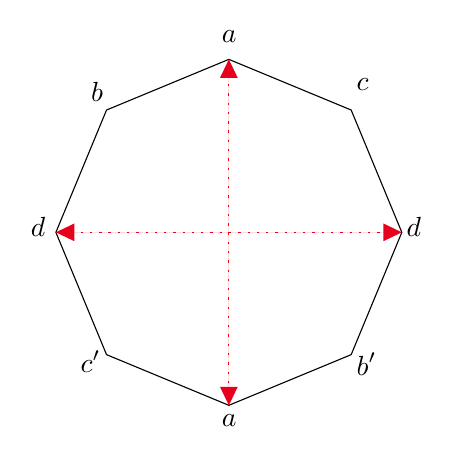
\begin{tikzpicture}[x=0.75pt,y=0.75pt,yscale=-1,xscale=1]
%uncomment if require: \path (0,300); %set diagram left start at 0, and has height of 300

%Shape: Regular Polygon [id:dp8058063624355654] 
\draw   (408,138.34) -- (383.59,197.27) -- (324.66,221.68) -- (265.73,197.27) -- (241.32,138.34) -- (265.73,79.41) -- (324.66,55) -- (383.59,79.41) -- cycle ;
%Straight Lines [id:da4976793908038122] 
\draw [color={rgb, 255:red, 255; green, 4; blue, 8 }  ,draw opacity=1 ][fill={rgb, 255:red, 240; green, 0; blue, 28 }  ,fill opacity=1 ] [dash pattern={on 0.84pt off 2.51pt}]  (324.66,58) -- (324.66,218.68) ;
\draw [shift={(324.66,221.68)}, rotate = 270] [fill={rgb, 255:red, 232; green, 1; blue, 29 }  ,fill opacity=1 ][line width=0.08]  [draw opacity=0] (8.93,-4.29) -- (0,0) -- (8.93,4.29) -- cycle    ;
\draw [shift={(324.66,55)}, rotate = 90] [fill={rgb, 255:red, 232; green, 1; blue, 29 }  ,fill opacity=1 ][line width=0.08]  [draw opacity=0] (8.93,-4.29) -- (0,0) -- (8.93,4.29) -- cycle    ;
%Straight Lines [id:da8020702890389528] 
\draw [color={rgb, 255:red, 232; green, 1; blue, 29 }  ,draw opacity=1 ][fill={rgb, 255:red, 232; green, 1; blue, 29 }  ,fill opacity=1 ] [dash pattern={on 0.84pt off 2.51pt}]  (244.32,138.34) -- (405,138.34) ;
\draw [shift={(408,138.34)}, rotate = 180] [fill={rgb, 255:red, 232; green, 1; blue, 29 }  ,fill opacity=1 ][line width=0.08]  [draw opacity=0] (8.93,-4.29) -- (0,0) -- (8.93,4.29) -- cycle    ;
\draw [shift={(241.32,138.34)}, rotate = 360] [fill={rgb, 255:red, 232; green, 1; blue, 29 }  ,fill opacity=1 ][line width=0.08]  [draw opacity=0] (8.93,-4.29) -- (0,0) -- (8.93,4.29) -- cycle    ;


% Text Node
\draw (320,225) node [anchor=north west][inner sep=0.75pt]   [align=left] {$\displaystyle a$};
% Text Node
\draw (320,40) node [anchor=north west][inner sep=0.75pt]   [align=left] {$\displaystyle a$};
% Text Node
\draw (385,195.27) node [anchor=north west][inner sep=0.75pt]   [align=left] {$\displaystyle b'$};
% Text Node
\draw (257,65) node [anchor=north west][inner sep=0.75pt]   [align=left] {$\displaystyle b$};
% Text Node
\draw (409,130) node [anchor=north west][inner sep=0.75pt]   [align=left] {$\displaystyle d$};
% Text Node
\draw (228,130) node [anchor=north west][inner sep=0.75pt]   [align=left] {$\displaystyle d$};
% Text Node
\draw (385,63) node [anchor=north west][inner sep=0.75pt]   [align=left] {$\displaystyle c$};
% Text Node
\draw (252,194) node [anchor=north west][inner sep=0.75pt]   [align=left] {$\displaystyle c'$};


\end{tikzpicture}

    \caption{$X'(2+4)$}
    \label{Skew-2}
\end{minipage}
\end{figure}

\section{The Known Examples}
Before proving that $\TC(\al,1-\al)$, $Q_2(\frac{1}{3})$, and $Q_2(\frac{1}{3})^\times \oplus \GenG{\id}$ are the only examples (up to isomorphism) of $2$-generated axial algebras of Monster type with skew axet $X'(1+2)$, it would be useful to show that they satisfy the conditions we desire. 
\subsection{Three Dimensions}
Let $A=\TC(\al)$ with $\al\notin \{0,1, \frac{1}{2},-1\}$. In \cite{mcinroy2022axial} and \cite{franchi20212}, this example has already been stated. Let $x,y,z$ be the distinct axes of $\mcal{J}(\al)$-type and notice that $\{x,y,z\}$ form a basis for $A$. The element $\id=\frac{1}{\al+1}(x+y+z)$ is the identity element of $A$. Letting $w=\id-x$, one can see that $w$ is an axis of $\mcal{J}(1-\al)$-type and $\al\id=(-w+y+z)$. Looking at $\GenA{w,y}$, we have
\begin{eqnarray*}
wy &=& (\id-x)y = y-\frac{\al}{2}(x+y-z) = y-\frac{\al}{2}(-w+\id +y-z)\\
&=&y-\frac{\al}{2}(-w+y-z)-\frac{1}{2}(-w+y+z) = \frac{\al+1}{2}w +\frac{1-\al}{2}(y-z).
\end{eqnarray*}
Hence $z\in \GenA{w,y}$ and $x$ is too. Therefore $A=\GenA{w,y}$. As $A$ is now of $\mcal{M}(\al,1-\al)$-type with respect to the axes $w$ and $y$, let the Miyamoto involutions of $w$ and $y$ be $\tau_w$ and $\tau_y$ respectively. As $y$ is of $\mcal{J}(\al)$-type, $\tau_y$ is the identity. On the other hand, one can check that $x\in A_0(w)$ and $y-z\in A_{1-\al}(w)$. Further,
\[ y = \frac{\al}{2}x + \frac{\al+1}{2}w +\frac{1}{2}(y-z)\]
and so
\[ y^{\tau_w}=\frac{\al+1}{2}w+\frac{\al}{2}x -\frac{1}{2}(y-z) =z.\]
Therefore $A$ is skew with axet $X'(1+2)$. To avoid confusion about fusion laws, we denote the skew algebra by $\TC(\al,1-\al)$.

\begin{rem}
If one used the same method to $\TC(\frac{1}{2})$, then it would produce the algebra $S(1)$. By Remark 5.9 and Lemma 5.12 in \cite{mcinroy2021forbidden}, $S(1)$ has axet $X(6)$.
\end{rem}

\subsubsection{A Variation}
One may notice that for $\TC(-1)$, we have only $\jor{-1}$-axes and no identity. It would be absurd to try to make an axial algebra of Monster type out of it. We therefore use $\TC(2)$ to produce an axial algebra with fusion law $\mon{-1,2}$. Take $A=\TC(2)$ with $\{u,v,w\}$ being the three distinct axes of $\jor{2}$-type. There is an identity in $A$, $\id=\frac{1}{3}(u+v+w)$. Let $y:=\id-u$ and $z:=\id-v$ be $\jor{-1}$-axes. Let us look at $\GenA{w,y}$. We get
\[wy=(\id-u)w=w-uw=w-(u+w-v)=v-u\]
and
\[y(u-v)=(\id-u)(u-v)=-v+uv=-v+(u+v-w)=u-w.\]
Hence $v-w\in \GenA{w,y}$ as well as $v\in \GenA{w,y}$. Further, $u\in \GenA{w,y}$ and so $A=\GenA{w,y}$. These axes now satisfy the fusion law of $\mon{-1,2}$. We have that $\tu{y}$ is trivial as it is a $\jor{-1}$-axis while $\tu{w}$ is not. The reader can check:
\begin{itemize}
    \item $w \in A_1(w)$,
    \item $\id-w =-(y+z)\in A_0(w)$, and
    \item $y-z \in A_2(w)$.
\end{itemize}
We have
\[ y= \frac{1}{2}(y+z)+\frac{1}{2}(y-z),\]
and 
\[ y^{\tu{w}}=\frac{1}{2}(y+z)-\frac{1}{2}(y-z)=z.\]
Therefore $A$ is skew with axet $X'(1+2)$, and denote this algebra by $\TC(-1,2)$.
\begin{note}
We have $yz=(\id-u)(\id-v)=\id-u-v+(u+v)-w=\id-w=-y-z$ and so $\GenA{y,z}\cong \TC(-1)^\times$, the $2$-dimensional quotient of $\TC(-1)$. This will be important in the proof later.
\end{note}
\begin{rem}
Another way to construct $\TC(-1,2)$ would be by attaching a universal identity to $\TC(-1)^\times$ (similar to the construction of $Q_2(\frac{1}{3})^\times \oplus \GenG{\id}$).
\end{rem}

\subsection{Four Dimensions}
Let $\F$ have characteristic not equal to $3$ and let $Q_2(\frac{1}{3})$ be defined as in \cite[Section 5.3]{galt2021double} with $\eta=\frac{1}{3}$. The algebra has a basis of two single axes, $s_1$ and $s_2$, and two double axes, $d_1$ and $d_2$ with the multiplication defined in Table \ref{mult Q}.
\begin{table}[b]
\begin{center}
    \begin{tabular}{c|c|c|c|c}
         & $s_1$ & $s_2$ & $d_1$ &$d_2$   \\
         \hline
        $s_1$ & $s_1$ &$0$& $\frac{1}{3}s_1+\frac{1}{6}d_1-\frac{1}{6}d_2$& $\frac{1}{3}s_1-\frac{1}{6}d_1+\frac{1}{6}d_2$\\
        \hline
        $s_2$ & & $s_2$ & $\frac{1}{3}s_2+\frac{1}{6}d_1-\frac{1}{6}d_2$& $\frac{1}{3}s_2-\frac{1}{6}d_1+\frac{1}{6}d_2$\\
        \hline
        $d_1$ &  &  & $d_1$&$-\frac{1}{3}s_1-\frac{1}{3}s_2+\frac{1}{3}d_1+\frac{1}{3}d_2$ \\
        \hline
        $d_2$ &  &  &  & $d_2$
    \end{tabular}
       \caption{The multiplication table of $Q_2(\frac{1}{3})$}
       \label{mult Q}
       \end{center}
\end{table}
\subsubsection{In characteristic not equal to 5}
When the field has characteristic not equal to $5$, $A=Q_2(\frac{1}{3})$ is simple by Theorem 1.6 in \cite{galt2021double} and has identity element, $\id = \frac{3}{5}(s_1+s_2+d_1+d_2)$. Notice  $s_1$ is a $\jor{\frac{1}{3}}$-axis while $d_1$ is a $\mon{\frac{2}{3},\frac{1}{3}}$-axis. Let $t_1:=\id-d_1$ and $t_2:=\id -d_2$. Then $t_1$ and $t_2$ are $\mcal{M}(\frac{1}{3},\frac{2}{3})$-axes. Let us look at $\GenA{t_1,s_1}$. We have that 
\[ s_1t_1 = s_1(\id -d_1)=s_1-\frac{1}{3}s_1-\frac{1}{6}d_1+\frac{1}{6}d_2 = \frac{2}{3}s_1-\frac{1}{6}d_1+\frac{1}{6}d_2= \frac{2}{3}s_1+\frac{1}{6}t_1-\frac{1}{6}t_2.\]
Therefore $t_2\in \GenA{s_1,t_1}$. Notice that $-\frac{1}{3}\id = s_1+s_2-t_1-t_2$. We have
\begin{eqnarray*}t_1t_2 = (\id-d_1)(\id-d_2) &=& \id -d_1-d_2+d_1d_2\\
&=& \id -\frac{1}{3}s_1-\frac{1}{3}s_2-\frac{2}{3}d_1-\frac{2}{3}d_2\\
&=& \id -\frac{1}{3}s_1-\frac{1}{3}s_2+\frac{2}{3}(\id-d_1)+\frac{2}{3}(\id-d_2)-\frac{4}{3}\id\\
&=&-\frac{1}{3}\id -\frac{1}{3}s_1-\frac{1}{3}s_2+\frac{2}{3}t_1+\frac{2}{3}t_2\\
&=& s_1+s_2-t_1-t_2 -\frac{1}{3}s_1-\frac{1}{3}s_2+\frac{2}{3}t_1+\frac{2}{3}t_2\\
&=& \frac{2}{3}s_1+\frac{2}{3}s_2-\frac{1}{3}t_1-\frac{1}{3}t_2.
\end{eqnarray*}
Hence $s_2$ and $\id$ are in $\GenA{s_1,t_1}$. Therefore $d_1,d_2\in \GenA{s_1,t_1}$ and so $A=\GenA{s_1,t_1}$ and has fusion law $\mon{\frac{1}{3},\frac{2}{3}}$. As $s_1$ is a $\jor{\frac{1}{3}}$-axis, $\tu{{s_1}}$ is the identity map.  The reader can check that:
\begin{itemize}
    \item $t_1 = \frac{1}{5}(3s_1+3s_2-2d_1+3d_2)\in A_1(t_1)$,
    \item $d_1 \in A_0(t_1)$, 
    \item $s_1+s_2-d_2 \in A_\frac{1}{3}(t_1)$, and
    \item $s_1-s_2 \in  A_\frac{2}{3}(t_1)$.
\end{itemize}
Hence
\[s_1 = \frac{5}{12}t_1+\frac{1}{6}d_1+\frac{1}{4}(s_1+s_2-d_2)+\frac{1}{2}(s_1-s_2).\]
Therefore
\[ s_1^{\tu{t_1}} = \frac{5}{12}t_1+\frac{1}{6}d_1+\frac{1}{4}(s_1+s_2-d_2)-\frac{1}{2}(s_1-s_2)=s_2.\]
Hence $A$ is skew with axet $X'(1+2)$. To avoid confusion with fusion laws, we denote this skew algebra by $Q_2(\frac{1}{3},\frac{2}{3})$. 
\begin{note}
One may think we can make any $Q_2(\eta)$, $\eta\notin \{-\frac{1}{2},\frac{1}{3}\}$, a skew axial algebra of Monster type with this method. This is partly possible if $\GenA{t_1,s_1}=Q_2(\eta)$. However the algebra would be skew but not of Monster type. The fusion law would have five elements and be an extension of the Monster fusion law.
\end{note}
\subsubsection{In characteristic 5}
Suppose now that the field has characteristic $5$. Then $\frac{1}{3}=-\frac{1}{2}$ and $Q_2(\frac{1}{3})$ is not simple by Theorem 1.6 in \cite{galt2021double}. This algebra has an annihilating element rather than an identity and so it is impossible with the technique used so far. We have that $I=\GenG{s_1+s_2+d_1+d_2}$ is the radical of $Q_2(\frac{1}{3})$. The quotient is denoted by $Q_2(\frac{1}{3})^\times$ and it is spanned by axes $\{x,y,z\}$ with their multiplication stated in Table \ref{mult Qx} (without the final row and column).
\begin{table}[b]
\begin{center}
    \begin{tabular}{c|c|c|c|c}
         & $x$ & $y$ & $z$ & $\id$   \\
         \hline
        $x$ & $x$ &$0$& $3x+y+2z$ & $x$\\
        \hline
        $y$ & & $y$ & $x+3y+2z$ & $y$\\
        \hline
        $z$ &  &  & $z$ & $z$\\
        \hline 
        $\id$ & & & & $\id$
    \end{tabular}
       \caption{The multiplication table of $Q_2(\frac{1}{3})^\times \oplus \GenG{\id}$}
       \label{mult Qx}
       \end{center}
\end{table}
The reader can check that $Q_2(\frac{1}{3})^\times =\GenA{x,z}$ with $x$ a $\jor{\frac{1}{3}}$-axis and $z$ a $\mon{\frac{2}{3},\frac{1}{3}}$-axis and so cannot be skew. In fact, this algebra has an axet of type $X(4)$. 

Let $A=Q_2(\frac{1}{3})^\times \oplus \GenG{\id}$ to be a $4$-dimensional algebra, where we add a universal identity element, $\id$, and multiplication is stated in Table \ref{mult Qx}. Let $w:=\id -z$ and let us look at $\GenA{x,w}$. Notice that
\[ wx=x(\id-z)=x - (3x+y+2z)=-2x-y-2z.\]
Therefore $y+2z\in \GenA{x,w}$ and we have
\[ w(y+2z)=wy=(\id-z)y=y-(x+3y+2z)=-x-2y-2z.\]
Hence $y+z\in \GenA{x,w}$. Moreover, $y,z \in \GenA{x,w}$ and so is $\id$. Therefore $A=\GenA{w,x}$. Showing that $x$ and $w$ are axes is a straightforward task as $x$ and $z$ are axes of the subalgebra $Q_2(\frac{1}{3})^\times$. We have that $x$ is a $\jor{\frac{1}{3}}$-axis and $w$ is a $\mon{\frac{1}{3},\frac{2}{3}}$-axis. Therefore $\tu{x}$ is trivial and $\tu{w}$ is not. For $w$, we have the following eigenvectors:
\begin{itemize}
    \item $w\in A_1(w)$,
    \item $z \in A_0(w)$,
    \item $x+y+3z \in A_{\frac{1}{3}}(w)$, and
    \item $x-y \in A_{\frac{2}{3}}(w)$. 
\end{itemize}
We have
\[ x= z+\frac{1}{2}(x+y+3z)+\frac{1}{2}(x-y)\]
and so
\[ x^{\tu{w}}=z+\frac{1}{2}(x+y+3z)-\frac{1}{2}(x-y)=y.\]
Therefore $A$ is skew with axet $X'(1+2)$. Further, $A\not\cong Q_2(\frac{1}{3})$ as $A$ has an identity element while $Q_2(\frac{1}{3})$ has not, in characteristic $5$. 

\begin{note}
One may think we can apply this method to $Q_2(-\frac{1}{2})^\times$ in characteristic not equal to $5$ to produce new algebras. This can be done however we run in the same problem as $Q_2(\eta)$ where the fusion law is an extension of the Monster fusion law and one needs to check that it is $2$-generated.
\end{note}
\section{The Foundations}
This section will be working closely with \cite[Section 4]{franchi20211} and \cite[Section 3]{rehren2017generalised}, which will be cited accordingly. We will state some of the results in those papers however we will omit the proofs.

Fix $(A,X)$ to be an $\mon{\al,\bt}$-axial algebra with $X=\{a_0,a_1\}$. For $i\in\{0,1\}$, let $\tu{i}$ be the Miyamoto involution associated to $a_i$. Let $\GenG{X}$ be isomorphic to $X'(1+2)$ and without loss of generality, let $\tu{0}$  be a non-trivial involution and $\tu{1}$ be equal to the identity. Set $a_{2i}:=a_0^{\tu{0}^i}$ and $a_{2i+1}:=a_1^{\tu{0}^i}$ for $i\in \Z$. Hence, 
\begin{equation}\label{axes rel}
    a_{2i}=a_0,\;\; a_{4i+1}=a_1,\;\; a_{4i-1}=a_{-1}\; \text{for} \;i \in \Z.
\end{equation} 
For $i\in \Z$ and $m\in \N$, define 
\begin{equation}\label{s rel}
 s_{i,m}:=a_ia_{i+m}-\bt(a_i+a_{i+m}).   
\end{equation} Let $f$ be the semi-automorphism of $A$ such that $a_i^f=a_{1-i}$ for all $i\in \Z$. This map is well-defined by Corollary 3.8 in \cite{franchi20211}. This $f$ is called the \emph{flip} and we do not assume it is an automorphism of $A$. Notice that $f$ has order $2$, $s_{0,1}^f=s_{0,1}$ and $s_{0,2}^f=s_{1,2}$. Using Definition \ref{Proj}, we define \[\lm_1:=\lm_{a_0}(a_1), \; \; \lmf_1:=\lm_{a_1}(a_0), \; \; \lm_2:=\lm_{a_0}(a_2)=1, \; \;\text{and }
\lmf_2:=\lm_{a_1}(a_{-1}).\]
To ease notation, we define the following constants:
\[ \gm:=\bt-\lm_1,\; \ep:=(1-\al)\lm_1-\bt, \; \dt:=(1-\al)\lm_1+\bt(\al-\bt-1).\]
In a similar fashion,
\[ \gm^f:=\bt-\lmf_1, \; \ep^f:=(1-\al)\lmf_1-\bt, \; \dt^f:=(1-\al)\lmf_1+\bt(\al-\bt-1).\]
They have the following relations:
\[
(\al-1)\gm=\ep+\al\bt=\dt+\bt^2\;\text{ and } \;(\al-1)\gm^f=\ep^f+\al\bt=\dt^f+\bt^2.
\]

\begin{lem}\label{axes sigma}
We have 
\begin{eqnarray*}
a_0s_{0,1}&=&(\al-\bt)s_{0,1}+\dt a_0 +\frac{1}{2}\bt(\al-\bt)(a_1+a_{-1})\\
a_1 s_{0,1}&=& (\al-\bt)s_{0,1}+ \dt^f a_1+\bt(\al-\bt) a_0 \\
a_{-1} s_{0,1} &=& (\al-\bt)s_{0,1} + \dt^f a_{-1}+\bt(\al-\bt) a_0.
\end{eqnarray*}
\proof The first two equalities are part of Lemma 3.1 in \cite{rehren2017generalised}. 
By the second equality, 
\[(a_1s_{0,1})^{\tu{0}} = [(\al-\bt)s_{0,1}+ \dt^f a_{1}+\bt(\al-\bt) a_0 ]^{\tu{0}}\]
if and only if
\[ a_{-1}s_{0,1} = (\al-\bt)s_{0,1}+ \dt^f a_{-1}+\bt(\al-\bt) a_0 \]
due to $\tu{0}$ being an automorphism of $A$. \qed
\end{lem}
\begin{lem}\label{sigma2}
We have that $s_{1,2}$ is in the span of $\{a_0,a_1,a_{-1}, s_{0,1}\}$.
\proof Applying $f$ to the first equality of Lemma 4.7 in \cite{franchi20211}, we get:
\begin{eqnarray*}
(\al-2\bt)a_1s_{0,2}&=&\bt^2(\al-\bt)(a_3+a_{-1})+2\bt(\al-\bt)s_{1,2}\\
&+&\left[-2\al\bt\lmf_1+2\bt(1-\al)\lm_1\right.\\
&+&\left.\frac{\bt}{2}(4\al^2-2\al\bt+4\bt^2-\al-2\bt)\right](a_0+a_2)\\
&+&\frac{1}{(\al-\bt)}\left[(6\al^2-8\al\bt-2\al+4\bt)(\lmf_1)^2\right.\\
&+&\left. 2\al(\al-1)\lm_1\lmf_1+2\al(-2\al-2\bt+1)(\al-\bt)\lmf_1\right.\\
&-&\left.4\bt(\al-1)(\al-\bt)\lm_1-\al\bt(\al-\bt)\lmf_2\right.\\
&+&\left.2\bt(2\al^2+\bt^2-\al)(\al-\bt)\right]a_1\\
&+&\left[-4\al\lmf_1-4(\al-1)\lm_1\right.\\
&+&\left.(4\al^2-2\al\bt+4\bt^2-\al-2\bt)\right]s_{0,1}.
\end{eqnarray*}
Applying relations in $(\ref{axes rel})$ and the fact that $s_{0,2}=a_0a_2-\bt(a_0+a_2)=(1-2\bt)a_0$ we get
\begin{eqnarray*}
(\al-2\bt)(1-2\bt)a_1a_0&=&2\bt^2(\al-\bt)a_{-1}+2\bt(\al-\bt)s_{1,2}\\
&+&2\left[-2\al\bt\lmf_1+2\bt(1-\al)\lm_1\right.\\
&+&\left.\frac{\bt}{2}(4\al^2-2\al\bt+4\bt^2-\al-2\bt)\right]a_0\\
&+&\frac{1}{(\al-\bt)}\left[(6\al^2-8\al\bt-2\al+4\bt)(\lmf_1)^2\right.\\
&+&\left. 2\al(\al-1)\lm_1\lmf_1+2\al(-2\al-2\bt+1)(\al-\bt)\lmf_1\right.\\
&-&\left.4\bt(\al-1)(\al-\bt)\lm_1-\al\bt(\al-\bt)\lmf_2\right.\\
&+&\left.2\bt(2\al^2+\bt^2-\al)(\al-\bt)\right]a_1\\
&+&\left[-4\al\lmf_1-4(\al-1)\lm_1\right.\\
&+&\left.(4\al^2-2\al\bt+4\bt^2-\al-2\bt)\right]s_{0,1}.\\
\end{eqnarray*}
Equivalently,
\begin{eqnarray*}
-2\bt(\al-\bt)s_{1,2}&=&2\bt^2(\al-\bt)a_{-1}\\
&+&2\left[-2\al\bt\lmf_1+2\bt(1-\al)\lm_1\right.\\
&+&\left.\frac{\bt}{2}(4\al^2-2\al\bt+4\bt^2-\al-2\bt)\right]a_0\\
&+&\frac{1}{(\al-\bt)}\left[(6\al^2-8\al\bt-2\al+4\bt)(\lmf_1)^2\right.\\
&+&\left.2\al(\al-1)\lm_1\lmf_1+2\al(-2\al-2\bt+1)(\al-\bt)\lmf_1\right.\\
&-&\left.4\bt(\al-1)(\al-\bt)\lm_1-\al\bt(\al-\bt)\lmf_2\right.\\
&+&\left.2\bt(2\al^2+\bt^2-\al)(\al-\bt)\right]a_1\\
&+&\left[-4\al\lmf_1-4(\al-1)\lm_1\right.\\
&+&\left.(4\al^2-2\al\bt+4\bt^2-\al-2\bt)\right]s_{0,1}\\
&-&(\al-2\bt)(1-2\bt)\left[s_{0,1}+\bt(a_0+a_1)\right].
\end{eqnarray*}
Therefore
\[ s_{1,2}=Pa_0+Qa_1+Ra_{-1}+Ss_{0,1}\]
where 
\begin{eqnarray*}
P&:=& \frac{1}{(\al-\bt)}\left[2(\al-1)\lm_1+2\al\lmf_1+\al(1-2\al)\right],\\
Q&:=&-\frac{1}{2\bt(\al-\bt)^2}\left[(6\al^2-8\al\bt-2\al+4\bt)(\lmf_1)^2+2\al(\al-1)\lm_1\lmf_1\right.\\
&+&\left.2\al(-2\al-2\bt+1)(\al-\bt)\lmf_1-4\bt(\al-1)(\al-\bt)\lm_1\right.\\
&-&\left.\al\bt(\al-\bt)\lmf_2+2\bt(2\al^2+\bt^2-\al)(\al-\bt)\right.\\
&-&\left.\bt(\al-\bt)(\al-2\bt)(1-2\bt)\right],\\
R&:=&-\bt, \text{ and}\\
S&:=&\frac{P}{\bt}.
\end{eqnarray*}
\qed
\end{lem}
\begin{lem}\label{mult lemma}
With the above notation, $Q=R$ and $a_1a_{-1}=P(a_0+\frac{1}{\bt}\sg)$.
\end{lem}
\proof
Since $s_{1,2}$ is invariant under $\tu{0}$, notice that 
\[0=(s_{1,2}-s_{1,2}^{\tu{0}})=(Q-R)(a_1-a_{-1})\]
To avoid a contradiction, $Q=R$ and so
\[ s_{1,2}=P\left(a_0+\frac{1}{\bt}s_{0,1}\right)-\bt(a_1+a_{-1}).\]
Hence
\[a_1a_{-1}= s_{1,2}+\bt(a_1+a_{-1})=P\left(a_0+\frac{1}{\bt}s_{0,1}\right).\] \qed
\begin{prop}\label{span prop}
We have $A$ is linearly spanned by $\mcal{B}=\{a_{-1},a_0,a_1,s_{0,1}\}$ and so is at most $4$-dimensional.
\proof From above, multiplication of $\mcal{B}$ has been described and shown to be in $\Span{\mcal{B}}$ except for $s_{0,1}^2$. If $\al\neq 2\bt$,  $s_{0,1}^2 \in \Span{\mcal{B}}$ by Lemma 4.7 in \cite{franchi20211}. 
If $\al = 2\bt$, by Lemma 3.5 in \cite{franchi20212}, $s_{0,1}^2$ is computed. As $s_{0,3}=s_{0,1}$ by Equation $(\ref{s rel})$, $s_{0,1}^2\in \Span{\mcal{B}}$.  \qed
\end{prop}

We will now state  Theorem 4.1.1 in \cite{rehren2015axial} where $R$ is a field. This is a extremely useful result that will be used multiple times in our reasoning. 
\begin{prop}[Rehren]\label{Rehren Thm}
Let $\al,\bt\notin \{0,1\}$ be distinct values. Suppose that $V=\GenA{p,q}$ be an axial algebra such that $p$ is a $\mcal{J}(\al)$-axis and $q$ is a $\mcal{J}(\bt)$-axis. Then $V\cong \TB$ or $V\cong \TC(\al,1-\al)$.
\end{prop}

\begin{rem}
In Rehren's proof, he only shows algebra isomorphisms of $V\cong \TC(\al)$ or $V\cong \TC(2)$ if $\al=-1$. However, for $\al\neq-1$, it is clear that $V\cong \TC(\al,1-\al)$ due $(V,\{p,q\})$ satisfying a fusion law $\mon{\al,1-\al}$. Further, for $\al=-1$, it is easy to show that $V\cong \TC(-1,2)$. Again, this is clear since $(V,\{p,q\})$ satisfies a fusion law $\mon{-1,2}$.  
\end{rem}

\section{Skew Relations}
To ease notation, set $a:=a_0$, $b:=a_1$, $c:=a_{-1}$, and $\sg:=s_{0,1}$. From Lemma \ref{axes sigma} and \ref{sigma2}, we have
\begin{eqnarray*}
a\sg&=&(\al-\bt)\sg+\dt a+\frac{1}{2}\bt(\al-\bt)(b+c),\\
b\sg&=& (\al-\bt)\sg+\bt(\al-\bt)a + \dt^f b,\\
c\sg&=& (\al-\bt)\sg+\bt(\al-\bt)a + \dt^f c,\\
 bc &=& P\left(a+\frac{1}{\bt}\sg\right).
\end{eqnarray*}
The last thing  to complete a multiplication table of $A$ is $\sg^2$. These expressions are in \cite{franchi20211} and \cite{franchi20212} for $\al\neq 2\bt$ and $\al=2\bt$ respectively. In this paper, we do not need the exact expression for $\sg^2$ and we simply write
\[ \sg^2 = \zt a + \te(b+c)+\kp \sg\]
with $\zt, \te, \kp \in \F$.
Notice that the $b$ and $c$ term are equal due to $\sg^2$ being invariant under $\tu{0}$ and Table \ref{mult table} gives us the complete multiplication of $A$.
\begin{table}[b]
\centering
\scalebox{0.9}{
    \begin{tabular}{c|c|c|c|c}
         & $a$ & $b$ & $c$ &$\sg$   \\
         \hline
        $a$ & $a$& $\bt a + \bt b + \sg$& $\bt a + \bt c+ \sg$& $\dt a+\frac{1}{2}\bt(\al-\bt)(b+c)+(\al-\bt)\sg$\\
        \hline
        $b$ & & $b$ & $P(a+\frac{1}{\bt}\sg)$ &$\bt(\al-\bt)a + \dt^f b+(\al-\bt)\sg$\\
        \hline
        $c$ &  &  & $c$& $\bt(\al-\bt)a + \dt^f c+(\al-\bt)\sg$\\
        \hline
        $\sg$ &  &  &  & $\zt a + \te(b+c)+\kp \sg$
    \end{tabular}}
\caption{The multiplication table of $A$}
\label{mult table}
\end{table}

The rest of this section will be producing results that will be used in the proof of Theorem \ref{Theorem}. First, we can calculate eigenspaces of $\text{ad}_a$ and $\text{ad}_b$.

\begin{lem}\label{eigen a}
The eigenspaces of $\text{ad}_a$ are the following:
\begin{enumerate}
    \item[$1$.] $\GenG{a}=A_1(a)$, 
    \item[$2$.] $\GenG{\ep a+\frac{1}{2}(\al-\bt)(b+c)-\sg}= A_0(a)$,
    \item[$3$.] $\GenG{\gm a +\frac{1}{2}\bt(b+c)+\sg}=A_\al(a)$, and
    \item[$4$.] $\GenG{b-c}= A_\bt(a)$.
\end{enumerate}
\proof See Lemma 4.4 in \cite{franchi20211}. \qed
\end{lem}
\begin{lem}\label{eigen b}
The eigenspaces of $\text{ad}_b$ are the following:
\begin{itemize}
    \item[$1$.] $\GenG{b}= A_1(b)$,
    \item[$2$.] $\GenG{-\frac{P}{\bt}a+Pb+c, (\al-\bt)a +\ep^fb-\sg}=A_0(b)$, and
    \item[$3$.] $\GenG{\bt a +\gm^fb+\sg}=A_\al(b)$.
\end{itemize}
\proof Using Table \ref{mult table}, the reader can check the generators are eigenvectors. As $A$ is at most $4$-dimensional, there are no more possible eigenvectors (up to linear combination). \qed 
\end{lem}
We can find certain relations from the conditions imposed by Lemma \ref{Seress}. To avoid focusing on how these relations are calculated, the reasoning is in the appendix for the reader to look at if they wish. 
\begin{lem}\label{skew rel}
We have that the following equations must hold:
\begin{equation}\label{proof1}
   \begin{split}
\lmf_2=-\frac{P}{\bt}\gm^f
\end{split} 
\end{equation} 
\begin{equation}\label{proof2}
    \begin{split}
\bt\dt =\frac{1}{2}\bt(\al-\bt)-\bt^2(\al-\bt)-(\al-2\bt)\dt^f.  
\end{split}
\end{equation} 
and
\begin{equation}\label{proof3}
\begin{split}
\frac{1}{2}(1-\bt)P=(\al-1)\gm^f.
\end{split}
\end{equation}

\end{lem}
\proof See the Appendix. \qed


\section{Proof of Theorem \ref{Theorem}}

Let $(A,X)$ be an $\mon{\al,\bt}$-axial algebra satisfying the hypothesis of Theorem \ref{Theorem} with $X=\{a,b\}$. By Proposition \ref{span prop}, we may assume that $A$ is spanned by $\{a,b,c,\sg\}$ and multiplication is defined in Table \ref{mult table}. We assume $b$ is a $\jor{\al}$-axis with $c=b^{\tu{a}}$. We set 
$U:=\GenA{b,c}$ which is a  $\jor{\al}$-axial algebra. The proof is split into two parts: $P=0$ or $P\neq 0$. 

\subsection{Orthogonal axes}\label{P zero}
For this section, we will assume that $P=0$.
By Table \ref{mult table}, $bc=0$; that is $U\cong \TB$. Hence $d:=b+c$ is a $\jor{2\al}$-axis in $A$. Notice that $d$ is not primitive as $A_1(d)=\GenG{b,c}$. Let $F:=A_{\{0,1,\al\}}(a)$ be the fixed subalgebra of $\tu{a}$. We have that $a,d,\sg \in F$ and $b-c\notin F$ which implies $\text{dim}F\leq\text{dim}A - 1\leq 3$.

\begin{lem}
We have $\al=\frac{1}{3}$, $F\cong \TC(\frac{1}{3},\frac{2}{3})$ or $F\cong \TC(\frac{2}{3},\frac{1}{3})$, and $A$ has dimension $4$.
\proof  One can show $F=\GenA{a,d}$ is a primitive axial algebra. We know $a$ satisfies $\jor{\al}$ fusion law and $d$ satisfies the $\jor{2\al}$ fusion law. As $\al\neq 2\al$, then $F\cong \TB$, $F\cong \TC(\frac{1}{3},\frac{2}{3})$, or $F\cong \TC(\frac{2}{3},\frac{1}{3})$ by Proposition \ref{Rehren Thm}. Let us assume $F\cong \TB$. Then $ad=0$ thus $\sg =-\bt a -\frac{\bt}{2}(b+c)$. Therefore the $\al$-eigenvector of $\text{ad}_a$ by Lemma \ref{eigen a} is now
\[ \gm a +\frac{1}{2}\bt(b+c)+\sg = (\gm-\bt)a=-\lm_1 a.\]
To avoid contradiction, we must have $\lm_1=0$ and $a$ is a $\jor{\bt}$-axis in $A$. By Proposition \ref{Rehren Thm}, $A\cong \TC(\al,1-\al)$ and $\id$ exists. Since $bc=0$, we must have $c=\id -b$ but that would make $c$ a $\jor{\bt}$-axis in $A$, which would contradict our axet. Therefore $\al=\frac{1}{3}$. We have $F\cong \TC(\frac{1}{3},\frac{2}{3})$ or $F\cong \TC(\frac{2}{3},\frac{1}{3})$. Since $F$ is $3$-dimensional, $A$ has to be $4$-dimensional. \qed
\end{lem}

\begin{lem}
We have that $A$ has fusion law $\mon{\frac{1}{3}, \frac{2}{3}}$ and multiplication is shown in Table $\ref{mult 4dim}$.

\proof As $P=0$, we have that $\gm^f=0$, moreover $\lmf_1=\bt$, by Equation (\ref{proof3}). Substituting into Equation (\ref{proof2}), we have
\[\bt \dt = \frac{1}{2}\bt(\al-\bt)-\bt^2(\al-\bt)+\bt^2(\al-2\bt)=\bt\left(\frac{1}{2}(\al-\bt)-\bt^2\right).\]
With $\al=\frac{1}{3}$, we get $\lm_1=\frac{1}{4}(\bt+1)$. Further, with $P=0$, we get
\[ 0=-\frac{4}{3}\lm_1+\frac{2}{3}\bt+\frac{1}{9}=-\frac{1}{3}(\bt+1)+\frac{2}{3}\bt+\frac{1}{9}=\frac{1}{3}\bt-\frac{2}{9}.\]
Therefore $\bt=\frac{2}{3}$.

With $F\cong \TC(\frac{1}{3},\frac{2}{3})$ or $F\cong \TC(\frac{2}{3},\frac{1}{3})$, there are exactly three $\mcal{J}(\frac{1}{3})$-axes in $F$, which are $a$ and two other elements, $e$ and $f$. Without loss of generality, let $e=\id -d$ where $\id=\frac{3}{4}(a+e+f)=3(a-d+f)$. Therefore $\{a,d,f,b\}$ is a basis for $A$ and by the multiplication of $F$, we have
\begin{eqnarray*}
ad&=&a(\id-e)=a-ae=a-\frac{1}{6}(a+e-f)=\frac{5}{6}a+\frac{1}{6}f-\frac{1}{6}(\id-d)\\
&=&\frac{5}{6}a+\frac{1}{6}f+\frac{1}{6}d-\frac{1}{2}(a-d+f)= \frac{1}{3}a +\frac{2}{3}d-\frac{1}{3}f,
\end{eqnarray*}
\begin{eqnarray*}
fd&=&f(\id-e)=f-fe=f-\frac{1}{6}(f+e-a)=\frac{5}{6}f+\frac{1}{6}a-\frac{1}{6}(\id-d)\\
&=&\frac{5}{6}f+\frac{1}{6}a+\frac{1}{6}d-\frac{1}{2}(a-d+f)= \frac{1}{3}f +\frac{2}{3}d-\frac{1}{3}a,
\end{eqnarray*}
and
\begin{eqnarray*}
af&=&\frac{1}{6}(a+f-e)=\frac{1}{6}(a+f+d-\id)\\
&=&\frac{1}{6}(a+f+d-3(a-d+f))= -\frac{1}{3}a+\frac{2}{3}d-\frac{1}{3}f. 
\end{eqnarray*}
Further,
\[ bd = b(b+c)=b+bc=b.\]
We have $ad =a(b+c)= 2\sg +\frac{4}{3} a +\frac{2}{3} d$, by the multiplication table of $A$, and so
\[ \sg =-\frac{1}{2}a -\frac{1}{6}f.\]
Hence 
\[ ab = \sg +\frac{2}{3} a +\frac{2}{3} b = \frac{1}{6}a-\frac{1}{6}f+\frac{2}{3} b.\] 
As $\lmf_1=\bt$, notice that $\frac{1}{6}a-\frac{2}{9} b +\frac{1}{6}f \in A_0(b)$ by Lemma \ref{eigen b}. Thus
\[
0 = b\left(a-\frac{4}{3}b +f\right) = \frac{1}{6}a -\frac{1}{6}f+\frac{2}{3} b -\frac{4}{3} b +bf\\
\]
which is equivalent to
\[
bf =-\frac{1}{6}a +\frac{1}{6}f+\frac{2}{3}b.
\]
Using $c=d-b$, we get the multiplication in Table \ref{mult 4dim}.\qed
\end{lem}
\begin{table}[ht]
\begin{center}
    \begin{tabular}{c|c|c|c|c}
         & $b$ & $c$ & $a$ &$f$   \\
         \hline
        $b$ & $b$ &$0$& $\frac{2}{3}b+\frac{1}{6}a-\frac{1}{6}f$& $\frac{2}{3}b-\frac{1}{6}a+\frac{1}{6}f$\\
        \hline
        $c$ & & $c$ & $\frac{2}{3}c+\frac{1}{6}a-\frac{1}{6}f$& $\frac{2}{3}c-\frac{1}{6}a+\frac{1}{6}f$\\
        \hline
        $a$ &  &  & $a$&$\frac{2}{3}b+\frac{2}{3}c-\frac{1}{3}a-\frac{1}{3}f$ \\
        \hline
        $f$ &  &  &  & $f$
    \end{tabular}
       \caption{The multiplication table of $A$ when $P=0$}
       \label{mult 4dim}
       \end{center}
\end{table}
\begin{lem}
Let $\F$ have characteristic not equal to $5$. Then $A\cong Q_2(\frac{1}{3},\frac{2}{3})$.
\proof We define the map $\varphi: A \rightarrow Q_2(\frac{1}{3},\frac{2}{3})$ with $\varphi(a)=t_1$, $\varphi(b)=s_1$, $\varphi(c)=s_2$, and $\varphi(f)=t_2$. The reader can check that this is an isomorphism. \qed
\end{lem}
\begin{lem}
Let $\F$ have characteristic equal to $5$. Then $A\cong Q_2(\frac{1}{3})^\times \oplus \GenG{\id}$. 
\proof We have the map $\phi: A \rightarrow Q_2(\frac{1}{3})^\times\oplus \GenG{\id}$ with $\phi(a)=\id-z$, $\phi(b)=x$, $\phi(c)=y$, and $\phi(\id)=\id$. This is a straightforward check that $\phi$ is an isomorphism. \qed
\end{lem}

\subsection{Non-Orthogonal Case}\label{P not zero}
We will now assume $P\neq 0$. As $U$ is a axial algebra of $\jor{\al}$-type, $U$ is either $\TB$, $S(2)^\circ$, $\TC(-1)^\times$ or $3$-dimensional. We should note that $S(2)^\circ$ is $\text{Cl}^0(\F^2,b)$ in \cite{hall2015primitive}. We will look at each possibility separately to complete our proof. We recommend the reader to \cite[Section 3]{hall2015primitive} and  \cite[Section 5]{mcinroy2021forbidden} for more information on $2$-generated axial algebras of Jordan type.

\begin{lem}
We have $U\not\cong \TB$. 
\proof Let $U\cong \TB$. As $P\neq 0$ then $\sg = -\bt a$. Then $A$ is at most $3$-dimensional. Notice that $ab = \bt b$. Therefore $b\in A_\bt(a)$ and we have that $c=b^{\tu{a}}=-b$. This is a contradiction as $c^2=(-b)^2=b\neq c$. \qed
\end{lem}
\begin{lem}\label{S2}
We have $U\not\cong S(2)^\circ$.
\end{lem}
\proof Let $U\cong S(2)^\circ$ and $bc=\frac{1}{2}(b+c)$. Further $bc=P(a+\frac{1}{\bt}\sg)$. Since $P\neq 0$, we can express $\sg$ in terms of $a$, $b$ and $c$. Thus
\[ \sg = \frac{\bt}{2P}(b+c)-\bt a.\]
Note that
\[ab =\frac{\bt}{2P}(b+c)+\bt b\;\text{ and }\;ac = \frac{\bt}{2P}(b+c)+\bt c.\]
Hence $(b+c)$ is an eigenvector of $\text{ad}_a$ with eigenvalue $\mu=\frac{\bt}{P}+\bt$. By $a$ being primitive and $\bt\neq 0$, $\mu\notin \{ 1, \bt\}$. Hence $\mu \in \{0,\frac{1}{2}\}$.

Suppose $\mu=\frac{1}{2}$ and so $(b+c)\in A_\frac{1}{2}(a)$. By the Monster fusion law, $(b+c)^2 \in A_{\{0,1\}}(a)$. However
\[ (b+c)^2=b+c+2bc=2(b+c)\in A_\frac{1}{2}(a).\]
Thus $b+c=0$ which contradicts our choice of $U$. 

Therefore $\mu=0$ and $a$ is a $\jor{\bt}$-axis in $A$. As $b$ is a $\jor{\frac{1}{2}}$-axis and by Proposition \ref{Rehren Thm}, $\frac{1}{2}+\bt=1$. Thus $\bt=\frac{1}{2}=\al$ which contradicts the fusion law. \qed
\begin{lem}
If $U\cong \TC(-1)^\times$, then $A\cong \TC(-1,2)$.
\proof Suppose $U\cong \TC(-1)^\times$. We will use a similar method to Lemma \ref{S2}. We have $bc= -(b+c)$ and $bc=P(a+\frac{1}{\bt}\sg)$ thus
\[ \sg = -\bt a -\frac{\bt}{P}(b+c)\] 
and $A$ is at most 3-dimensional. Note that
\[ ab = -\frac{\bt}{P}(b+c)+\bt b\; \text{ and }\; ac = -\frac{\bt}{P}(b+c)+\bt c.
\]
Hence $(b+c)$ is an eigenvector of $\text{ad}_a$ with eigenvector $\mu=-\frac{2\bt}{P}+\bt$. Note that $\mu\notin \{1,\bt\}$ as it would contradict $a$ being primitive and $\bt\neq 0$ respectively. Thus $\mu \in \{0,-1\}$.

Suppose $\mu=-1$ moreover $(b+c)\in A_{-1}(a)$. By the Monster fusion law, $(b+c)^2\in A_{\{1,0\}}(a)$. However
\[ (b+c)^2=b+c+2bc=-(b+c)\in A_{-1}(a).\]
Thus $b+c=0$ which contradicts $U$.

Therefore $\mu=0$ and $a$ is $\jor{\bt}$-axis and by Proposition \ref{Rehren Thm}, we get $\bt=2$ and $A\cong \TC(-1,2)$. \qed
\end{lem}
If $U$ is $3$-dimensional, then $U$ is either $\TC(\al)$, $S(\dt)$ with $\dt\neq 2$ (denoted by $\text{Cl}^J(\F^2,b)$ in \cite{hall2015primitive}) or $\widehat{S}(2)^\circ$ (denoted by $\text{Cl}^{00}(\F^2,b)$ in \cite{hall2015primitive}).  

\begin{lem}
Let $U$ be $3$-dimensional, then $A=U$. Further, $U\cong \TC(\al)$ and $A\cong \TC(\al,1-\al)$ for $\al\neq -1$.
\proof Assume for a contradiction that $A\neq U$. Therefore $A$ is 4-dimensional with basis $\{a,b,c,\sg\}$. By Lemma \ref{eigen b}, we have
\begin{eqnarray*}
-\frac{P}{\bt}a +P b +c \in A_0(b)\text{ and } \bt a +\gm^f b +\sg \in A_\al(b).
\end{eqnarray*}
By the fusion law, the product of these two vectors will be in $A_\al(b)=\GenG{\bt a +\gm^fb +\sg}$ moreover the $c$ component is zero. We have
\begin{eqnarray*}
\left[-\frac{P}{\bt}a +P b +c \right]\left[\bt a +\gm^f b +\sg\right] &=& -Pa -\frac{P}{\bt}\gm^fab -\frac{P}{\bt}a\sg +P\bt ab\\
&+&P\gm^f b +Pb\sg +\bt ac +\gm^fbc +c\sg\\
&=&[...]a + [...]b+ [...]\sg\\
&+& \left[-\frac{1}{2}(\al-\bt)P+\bt^2+\dt^f\right]c.
\end{eqnarray*}
Thus
\[ \frac{1}{2}(\al-\bt)P =(\al-1)\gm^f.\]
However by Equation (\ref{proof3}), we get
\[\frac{1}{2}(\al-\bt)P =(\al-1)\gm^f  = \frac{1}{2}(1-\bt)P\]
which implies that $\al=1$. A contradiction and so $U=A$. 

The possible options for $U$ (and $A$) are $S(\dt)$ with $\dt\neq 2$, $\widehat{S}(2)^\circ$ and $\TC(\al)$. Let us look at each algebra separately.

Suppose $U\cong S(\dt)$. This is the same algebra in Section  3.5 of \cite{hall2015primitive}. It is shown that all non-trivial idempotents in $U$ have fusion law $\jor{\frac{1}{2}}$ and so $a$ must be a $\jor{\frac{1}{2}}$-axis in $A$. Thus $A_\bt(a)=\{0\}$ and the axet is not skew. 

Suppose $U\cong \widehat{S}(2)^\circ$. This is discussed in Section 5 of \cite{mcinroy2021forbidden}. We have that every non-trivial idempotent in $U$ is a $\jor{\frac{1}{2}}$-axis. As before, we get $A_\bt(a)=\{0\}$ and the axet cannot be skew. 

Therefore $U\cong \TC(\al)$. If $\al\neq-1$, then we get $A\cong \TC(\al,1-\al)$. If $\al= -1$, $A$ is not skew.  \qed
\end{lem}
As we have exhausted all the cases for $P=0$ and $P\neq 0$, this completes the proof of Theorem \ref{Theorem}.


\section{Proof of Corollary \ref{Corollary}}
Let $A=\GenA{p,q}$ where $p$ is a $\mon{\al,\bt}$-axis and $q$ is a $\jor{\al}$-axis. 

Suppose that $q$ is fixed by $\tu{p}$. Both $p,q\in A_{\{0,1,\al\}}(p)$ and by the properties of $\mon{\al,\bt}$, we cannot produce a non-zero element in $A_\bt(p)$. Hence $p$ is a $\jor{\al}$-axis and so $A$ is an axial algebra of $\jor{\al}$-type. 

Now suppose $q$ is not fixed by $p$ and say $q^{\tu{p}}=r$ where $r$ is another axis. By $\tu{p}$ being an automorphism, $r$ is a $\jor{\al}$-axis and $\GenG{p,q}=\{p,q,r\}\cong X'(1+2)$. Therefore $A$ has skew axet of $X'(1+2)$ and is listed in Theorem \ref{Theorem}. 

\section{Larger Skew Axets}
For the majority of this paper, we have set the axet of $(A,X)$ to be $X'(1+2)$. In this section, we will look at larger skew axets and see if our work can simplify their classification.

To remind the reader, let $k\in \N$ and $k>1$. We have the axet of $X'(k+2k)$ to be the axet $X(4k)$ with the extra condition: for $i\in \Z$, $a_{2i}=a_{2(i+k)}$. We do not relabel the vertices when it becomes skew. Therefore,
\[ X(4k):=\{ a_i \; | \; i \in \Z \;\text{ and } \; a_i=a_{i+4k}\}\]
and 
\[ X'(k+2k):=\{ a_i \in X(4k) \; | \; a_{2j}=a_{2(j+k)} \; \forall j \in \Z\}.\]
Looking at the Miyamoto involution of either $X(4k)$ and $X'(k+2k)$, we have that for $i,j\in \Z$, 
\[ a_i^{\tu{j}}= a_{2j-i}.\]
\subsection{The Odd Case}
We will now present a result that M\textsuperscript{c}Inroy suggested.
\begin{prop}\label{odd k}
Let $k$ be odd. For axet $X'(k+2k)$, there exists a subaxet which is isomorphic $X'(1+2)$. 
\proof As $k$ is odd, $a_k$ is in the odd orbit and  $ a_0^{\tu{k}}= a_{2k-0}=a_0$. Therefore $a_0$ is fixed by $\tu{k}$. We have that  $a_k^{\tu{0}}= a_{0-k}=a_{-k}$. Therefore the set $Y=\{a_0,a_k,a_{-k}\}=\GenG{a_0,a_k}$ is a skew axet and is isomorphic to $X'(1+2)$. \qed
\end{prop}
\begin{cor}\label{odd cor}
    Let $k>1$ be odd and $(A,X)$ be a $2$-generated $\mon{\al,\bt}$-axial algebra with skew axet $X'(k+2k)$. Then $\al+\bt=1$. Further, either $A$ has a subalgebra isomorphic to either $\TC(\al,1-\al)$, $Q_2(\frac{1}{3},\frac{2}{3})$ or $Q_2(\frac{1}{3})^\times \oplus \GenG{\id}$.

\proof  By Proposition \ref{odd k}, $X$ must contain a subaxet, $Y=\GenA{a_0,a_k}$, isomorphic to $X'(1+2)$. Let $B=\GenA{a_0,a_k}$ be the $2$-generated axial algebra of Monster type with axet $Y$. As $B$ is generated by two axes in $A$, then $A$ shares the same fusion law in $B$. By Theorem \ref{Theorem}, the rest follows. \qed
\end{cor}

Let $k>1$ and be odd. By Proposition \ref{odd k} and Corollary \ref{odd cor}, we have a possibly strategy to classify all $2$-generated axial algebras of Monster type with skew axet $X'(k+2k)$. Suppose $(A,X)$ has our desired conditions. Notice that $L=\GenA{a_1,a_{-1}}$ is a $2$-generated axial algebra of Monster type. Further, $\tu{0}$ acts as the flip automorphism of $L$ thus $L$ is symmetric. By the classification of $2$-generated symmetric axial algebras of Monster type in \cite{yabe2023classification}, \cite{franchi2022classifying} and \cite{franchi2022quotients} together with the conditions from Corollary \ref{odd cor}, we will have a short list for possible options of $L$. 

We will complete this case in a second paper, going into much more detail. Moreover, we will look at when $k$ is even and progress to completely classifying skew axial algebras of Monster type. 
\appendix
\section{Skew Equations}
We will justify and show the three equations used in Lemma \ref{skew rel} to narrow our search for these skew axial algebras. Although they do not provide much use to understanding how these algebras could be constructed, they do make the proof easier.

Suppose $v$ is an $\mu$-eigenvector of an axis, $x$, where $\mu\neq1$. Then the projection on that axis should be equal to 0; that is, $\lm_x(v)=0$. Coincidentally, nearly all of the eigenvectors in Lemma \ref{eigen a} and \ref{eigen b} satisfy that rule. However we have
\begin{equation*}
 0=\lm_b\left(-\frac{P}{\bt}a+Pb+c\right) = -\frac{P}{\bt}\lmf_1+P+\lmf_2.
\end{equation*}
Whence we get Equation (\ref{proof1}).

\begin{defn}
Let $x$ be a $\mon{\al,\bt}$-axis in $A$, $\lm\in \{1,0, \al, \bt\}$ and $v\in A$. We denote $[v]^x_\lm$ to be the component of $v$ in $ A_\lm(x)$. 
\end{defn}
\begin{lem}
Let $w:=\frac{1}{2}(b-c)$. We have $[a]^a_\bt=0$, $[b]^a_\bt=w$, $[c]^a_\bt=-w$, $[\sg]^a_\bt=0$. Further, $[ab]^a_\bt=\bt w$, $[ac]^a_\bt=-\bt w$, $[bc]^a_\bt=0$, $[a\sg]^a_\bt=0$, $[b\sg]^a_\bt=\dt^fw$, $[c\sg]^a_\bt=-\dt^fw$ and $[\sg^2]^a_\bt=0$.
\end{lem}
\proof
As $a\in A_1(a)$, it has no $\bt$-component in $A_\bt(a)$ and $[a]^a_\bt=0$. As $\sg\in A_{\{1,0,\al\}}(a)$, it has no $\bt$-component in $A_\bt(a)$ and $[\sg]^a_\bt=0$. We can express $b$ in terms of the eigenvectors of $\text{ad}_a$ in Lemma \ref{eigen a}. The reader can check
\[ b= \lm_1 a+ \frac{1}{\al}\left(\ep a+\frac{1}{2}(\al-\bt)(b+c)-\sg\right)+ \frac{1}{\al}\left(\gm a +\frac{1}{2}\bt(b+c)+\sg\right)+\frac{1}{2}(b-c).\]
Thus $[b]_\bt^a=w$. As $c=b^{\tu{a}}$, we get $[c]_\bt^a=-w$.

Let $x, y \in A_{\{0,1,\al\}}(a)$ and notice $x^2, xy\in A_{\{1,0,\al\}}(a)$ and so has no $\bt$-component in $A_\bt(a)$. Therefore $[\sg^2]^a_\bt=[a\sg]^a_\bt=0$. Also
\[ [bc]_\bt^a=P\left([a]_\bt^a+\frac{1}{\bt}[\sg]_\bt^a\right)=0.\]
Note that
\[ [ab]_\bt^a=[\sg]_\bt^a+\bt[a]_\bt^a+\bt[b]_\bt^a=\bt w\]
and 
\[ [b\sg]_\bt^a=(\al-\bt)[\sg]_\bt^a+\bt(\al-\bt)[a]_\bt^a+dt^f[b]_\bt^a=\dt^f w.\]
Applying $\tu{a}$, we get $[ac]_\bt^a$ and $[c\sg]_\bt^a$. \qed



Let $u:= (b -\al)a - \bt b=\sg -(\al-\bt)a$. As $A_\bt(b)=\{0\}$, we have that $u\in A_{\{1,0\}}(b)$. By Lemma \ref{Seress}, the following holds
\[b(au)=(ba)u.\]
Notice
\[ au = a(\sg -(\al-\bt)a)=(\dt -(\al-\bt))a+\frac{1}{2}\bt(\al-\bt)(b+c)+(\al-\bt)\sg\]
and so
\begin{eqnarray*}
[b(au)]_\bt^a &=& (\dt -(\al-\bt))[ab]_\bt^a+\frac{1}{2}\bt(\al-\bt)([b]_\bt^a+[bc]_\bt^a)+(\al-\bt)[b\sg]_\bt^a\\
& =& \left(\bt(\dt -(\al-\bt))+\frac{1}{2}\bt(\al-\bt)+(\al-\bt)\dt^f\right)w
\end{eqnarray*}
We also have 
\begin{eqnarray*}
[(ba)u]_\bt^a&=&[(\sg+\bt a +\bt b)(\sg -(\al-\bt)a)]_\bt^a\\
&=& [\sg^2]_\bt^a -(\al-2\bt)[a\sg]_\bt^a +\bt [b\sg]_\bt^a -\bt(\al-\bt)[a]_\bt^a - \bt(\al-\bt)[ab]_\bt^a\\
&=& (\bt\dt^f -\bt^2(\al-\bt)) w
\end{eqnarray*}
By Lemma \ref{Seress}, we have $0=(ba)u-b(au)$ moreover $0=[(ba)u]_\bt-[b(au)]_\bt$. Looking at the coefficient of $w$, we have
\begin{eqnarray*} 
0&=& (\bt\dt^f-\bt^2(\al-\bt))\\
& -& \left(\bt \dt -\bt(\al-\bt)+\frac{1}{2}\bt(\al-\bt)+(\al-\bt)\dt^f\right)\\
&=&-\bt^2(\al-\bt) -\bt\dt+\frac{1}{2}\bt(\al-\bt)-(\al-2\bt)\dt^f.
\end{eqnarray*}
Rearranging we get Equation (\ref{proof2}).

Let $v:=Pa+\frac{P}{\bt}\sg -\al c=c(b-\al)$. Notice that $v \in A_{\{1,0\}}(b)$. Again by Lemma \ref{Seress}, the following holds
\[b(av)=(ba)v.\]
We have
\begin{eqnarray*}
av &=& Pa +\frac{P}{\bt}\left(\dt a + \frac{1}{2}\bt(\al-\bt)(b+c) +(\al-\bt)\sg\right)\\
& -&\al(\bt a +\bt c +\sg)\\
&=&\left(P +\frac{P}{\bt}\dt -\al\bt\right)a+\left(\frac{1}{2}(\al-\bt)P\right)b\\
&+&\left(\frac{1}{2}(\al-\bt)P-\al\bt\right)c+\left(\frac{P}{\bt}(\al-\bt)-\al\right)\sg.
\end{eqnarray*}
Therefore
\begin{eqnarray*}
[b(av)]_\bt^a &=&\left(P +\frac{P}{\bt}\dt -\al\bt\right)[ab]_\bt^a+\left(\frac{1}{2}(\al-\bt)P\right)[b]_\bt^a\\
&+&\left(\frac{1}{2}(\al-\bt)P-\al\bt\right)[bc]_\bt^a+\left(\frac{P}{\bt}(\al-\bt)-\al\right)[b\sg]_\bt^a.\\
&=&\left(\bt \left(P +\frac{P}{\bt}\dt -\al\bt\right)+\dt^f\left(\frac{P}{\bt}(\al-\bt)-\al\right)\right)w
\end{eqnarray*}
We also have
\begin{eqnarray*}
[(ba)v]_\bt^a&=&\left[\left(\bt a +\bt b +\sg\right)\left(Pa+\frac{P}{\bt}\sg -\al c\right)\right]_\bt^a\\
&=&2P[a\sg]_\bt^a +\frac{P}{\bt}[\sg^2]_\bt^a -\al [c \sg]_\bt^a + \bt P [a]_\bt^a -\al\bt [ac]_\bt^a\\
&+&\bt P [ab]_\bt^a +P[b\sg]_\bt^a -\al\bt [bc]_\bt^a\\
&=&\left(\al \dt^f +\al\bt^2 +\bt^2 P  +P\dt^f\right)w
\end{eqnarray*}
By Lemma \ref{Seress}, $0=[b(av)]^a_\bt-[(ba)v]^a_\bt$ and looking at the coefficient of $w$, we get 
\begin{eqnarray*}
0&=&[b(av)]_\bt-[(ba)v]_\bt\\
&=&\left(\bt P +\dt P -\al\bt^2+\frac{1}{2}(\al-\bt)P+\frac{P}{\bt}(\al-\bt)\dt^f -\al\dt^f\right)\\
&-&\left(\bt^2P +P\dt^f+\al\dt^f +\al\bt^2 \right)\\ 
&=&\left(\frac{P}{\bt}\left[\bt^2 +\bt\dt+\frac{1}{2}\bt(\al-\bt)+(\al-2\bt)\dt^f-\bt^3\right]-2\al(\dt^f+\bt^2)\right).
\end{eqnarray*}
From Equation (\ref{proof2}), we get that
\begin{eqnarray*}
0&=&\frac{P}{\bt}\left[\bt^2 -\bt^2(\al-\bt) +\frac{1}{2}\bt(\al-\bt)-(\al-2\bt)\dt^f\right.\\
&+&\left.\frac{1}{2}\bt(\al-\bt)+(\al-2\bt)\dt^f-\bt^3\right]-2\al(\dt^f+\bt^2)\\
&=&\frac{P}{\bt}\left[\bt^2 -\bt^2(\al-\bt) +\bt(\al-\bt)-\bt^3\right]-2\al(\dt^f+\bt^2)\\
&=&\frac{P}{\bt}\al\bt\left[1-\bt\right]-2\al(\dt^f+\bt^2).
\end{eqnarray*}
Hence we get Equation (\ref{proof3}).

\section*{Acknowledgements}
I would like to thank Professor Sergey Shpectorov for his guidance throughout my PhD studies so far and pushing me to complete this paper. I would also like to thank my family for their continuing support. 
\bibliographystyle{abbrv}
\bibliography{references}
\end{document}
